% ----------------------------------------------------------------------
%  *** DOCUMENT INFO ***
%
% Title: IHM-Labo-02
% Matière: IHM
% Auteur: Sébastien Richoz & Damien Rochat
% ----------------------------------------------------------------------
\documentclass[11pt, a4paper, french]{article}

% -----------------------------------------------------------------------
% *** PACKAGES ***
% -----------------------------------------------------------------------
\usepackage[utf8]{inputenc} % encodage accent
\usepackage[T1]{fontenc} % encodage accent
\usepackage{ae, pslatex} % Joli output en PDF
\usepackage[french]{babel} % Renomme les noms des chapitres, dates, ...
\usepackage{listings} % pour highlighter du code mySQL
\usepackage{listingsutf8}
\usepackage{xcolor}
\usepackage{graphicx} % Pour gérer des images
\usepackage{fancyhdr} % En-têtes améliorés
\usepackage{multicol}
\usepackage{vmargin}
\usepackage{etoolbox} % structure if else simplifiée

% -----------------------------------------------------------------------
%  *** CONFIGS ***
% -----------------------------------------------------------------------
\definecolor{LightGray}{gray}{0.9}
\definecolor{codegreen}{rgb}{0,0.6,0}
\definecolor{codegray}{rgb}{0.5,0.5,0.5}
\definecolor{codepurple}{rgb}{0.58,0,0.82}
\graphicspath{ {images/} } % Chemin des images

\usepackage[pdftex, % metadata fichiers pdf
			pdftitle={IHM Labo 02},
			pdfauthor={Sébastien Richoz, Damien Rochat},
			pdfsubject={Rapport IHM Labo 02}]{hyperref}

\setlength\parindent{0pt} % pas d'indentation de la première ligne des paragraphes


% -----------------------------------------------------------------------
%  *** MARGES ***
% -----------------------------------------------------------------------
%\addtolength{\textwidth}{170pt} \addtolength{\hoffset}{-85pt}
%\addtolength{\textheight}{150pt} \addtolength{\voffset}{-75pt}

\setpapersize{A4}
\setmarginsrb{40pt}{24pt}{40pt}{24pt}{14pt}{24pt}{14pt}{24pt}
%\setmarginsrb{a}{b}{c}{d}{e}{f}{g}{h}
%
% a => left margin
% b => top margin
% c => right margin
% d => bottom margin
% e => header height
% f => distance between header and text
% g => footer height
% h => distance between bottom page and bottom footer


% -----------------------------------------------------------------------
%  *** EN-TETE ET PIED DE PAGE ***
% -----------------------------------------------------------------------
\pagestyle{fancy}

\renewcommand{\sectionmark}[1]{\markright{\thesection\ #1}} % Noms des sections en minuscule
\fancyhf{}  												% Supprime les entetes et pieds existants

\fancyhead[L]{IHM-Labo-02}  % titre
\fancyfoot[C]{Page \thepage}  							% N° de la page
\fancyfoot[L]{Sébastien Richoz \& Damien Rochat}		% pieds de page	
\fancyfoot[R]{Novembre 2016}							% date
\renewcommand{\headrulewidth}{0.5pt}
\renewcommand{\footrulewidth}{0.5pt}

% -----------------------------------------------------------------------
%  *** TITRE ***
% -----------------------------------------------------------------------
\title{IHM Labo 02}
\author{Sébastien Richoz, Damien Rochat}
\date{Novembre 2016}

% ****************************************************************************************************************
% --- DOCUMENT PRINCIPAL ---
% ****************************************************************************************************************
\begin{document}
	\maketitle

	\part*{Interface}
		 L'interface de l'application permet à l'utilisateur d'aller de haut en bas, comme le fait naturellement une personne lorsqu'elle regarde quelque chose. \\
		 
		 L'utilisateur a tout d'abord la possibilité de sélectionner une vidéo, en passant par le bouton \textbf{Open video} ou en cliquant dans la grande zone centrale, comme les personnes en ont l'habitude lorsqu'une icône semblable (représentant un upload) est visible. Une fois la vidéo sélectionnée, ses informations sont affichées et la vidéo peut être lue. Ceci simplifie grandement la manière de trouver les passages recherchés. \\
		 
		 Les composants suivants permettent de définir la coupure que l'ont souhaite. Deux manières sont proposées à l'utilisateur, soit en passant par le "double slider" ou alors en passant par les boutons \textbf{plus} et \textbf{moins} respectifs pour modifier le début ou la fin de la vidéo. La visualisation de la vidéo est automatiquement mise à jour afin que l'utilisateur puisse être le plus précis possible. La durée de la vidéo résultante est également affichée, ce qui peut être utile dans le cas où une personne a une durée limite. \\
		 
		 La troisième étape pour l'utilisateur est de retrouver la commande ffmpeg qui lui permettra de couper sa vidéo. Avec les chemins absolus vers les vidéos, la commande devenait beaucoup trop grande à afficher, nous avons donc choisi de les masquer dans la commande, mais avons mis en place un bouton permettant de copier la commande complète dans le presse papier de l'utilisateur. Pour ne pas perturber l'utilisateur, nous lui informons que ces chemins relatifs sont bel et bien copiés au moyen d'un texte explicatif en dessous de la commande, et lui affichons explicitement ces chemins.
		 
		 \begin{center}
		 	\makebox[\textwidth]{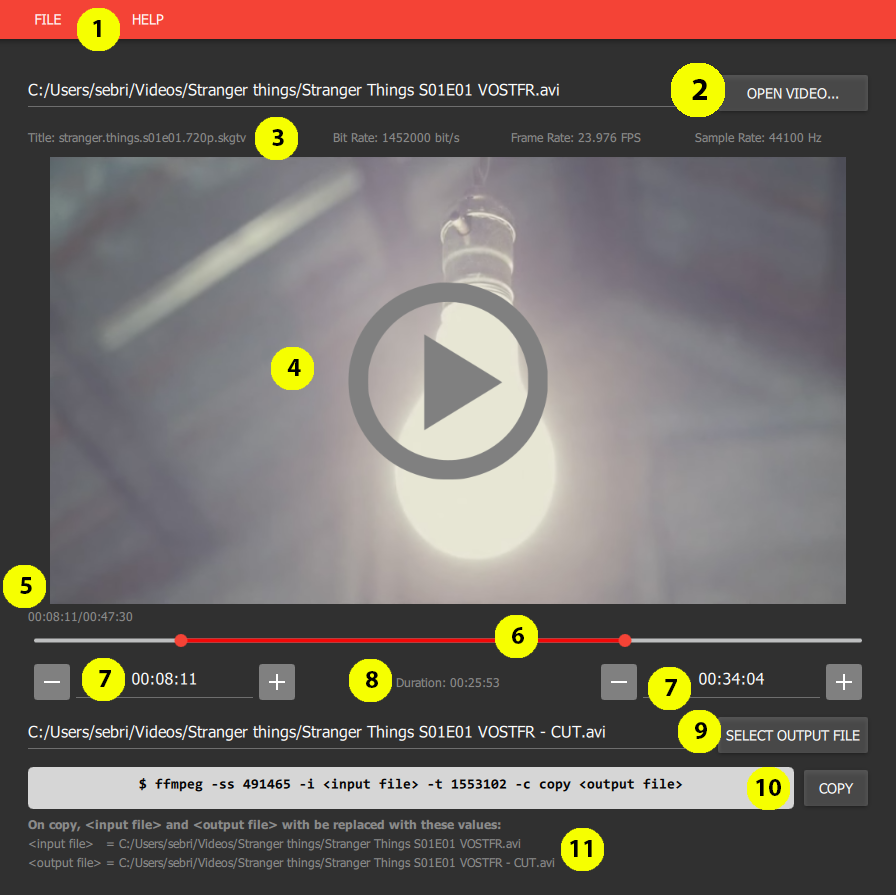
\includegraphics[width=\textwidth]{screenshot.PNG}}
		 \end{center}
	 \begin{enumerate}
	 	\item Menu de l'application
	 	\item Champ texte permettant d'éditer le chemin de la vidéo et bouton OPEN VIDEO... pour l'ouvrir à partir du navigateur de fichier natif au système d'exploitation
	 	\item Informations sur la vidéo: Titre, Nombre de bit par seconde, Nombre d'images par seconde, Taux d'échantillonnage
	 	\item écran vidéo : lorsqu'il n'y a pas de vidéo, une icône cliquable est affichée pour en charger une. Lorsqu'il y a une vidéo, l'icône play ci-dessus est affiché pour jouer la vidéo. Une fois la vidéo en pause, l'icône play s'affiche à nouveau.
	 	\item La position actuelle de la vidéo par rapport à sa durée totale exprimé ici selon le format hh:mm:ss/hh:mm:ss
	 	\item Le "Double Slider" permettant de sélectionner une partie de la vidéo. La partie en rouge met en évidence la portion sélectionnée. Les deux points sont "drag'n'dropable" et permettent de modifier cette portion.
	 	\item Les deux champs spécifiant la position de départ et de fin de la vidéo à séquencer. En interagissant avec les boutons + et -, le double slider et la vidéo s'adaptent.
	 	\item Ici figure la durée totale de la portion sélectionnée
	 	\item Le champ permet de saisir un fichier de sortie, alors que le bouton "SELECT OUTPUT FILE" permet d'ouvrir l'explorateur de fichier natif à l'OS pour en chercher un.
	 	\item La commande ffmpeg résultante du découpage vidéo avec les fichiers d'entrée et de sortie. Les temps y sont affichés en millisecondes. Le boutons "COPY" est désactivé tant que les deux fichiers d'entrée et de sorties ne sont pas choisis.
	 	\item L'information "On copy, ..." expliquant à l'utilisateur que c'est bien la commande complète qui va être copiée.
	 \end{enumerate}
 
	\part*{Erreurs gérées}
		Voici la liste des erreurs que l'application traitent actuellement :
		\begin{itemize}
			\item Le fichier d'entrée n'existe pas ou son format n'est pas supporté.
			\item Le fichier de sortie n'est pas correct.
			\item La fin de la coupure doit se trouver après son commencement.
			\item Le bouton de copie de la commande dans le presse papier ne peut être utilisé que lorsque une vidéo d'entrée et une de sortie sont spécifiées.
		\end{itemize}

	\part*{Améliorations}
		Actuellement, la visualisation de la vidéo s'adapte en fonction des configurations de l'utilisateurs. Il serait utile d'ajouter un nouveau contrôleur afin de pouvoir se déplacer dans la vidéo sans que cela n'influence les paramètres de coupe. \\
		
		Une autre chose est que les temps utilisés afin de définir le début et la fin de la vidéo vont à la seconde près. Alors qu'une vidéo contient encore plusieurs images par secondes. Cette précision pourrait être améliorée en se basant sur le FPS (Frame Per Second) de chaque vidéo. \\
		
		Certains format de vidéo ne sont pas pris en charge. Les modules Qt Quick sont encore très récents et ceux-ci vont être améliorés à l'avenir.
	
\end{document}
